\subsection{Examples of Trajectories}

\subsubsection{Straight Line Trajectory}
Consider the following diagram
\begin{mycenter}
	\tikzset{every picture/.style={line width=0.75pt}} %set default line width to 0.75pt        

	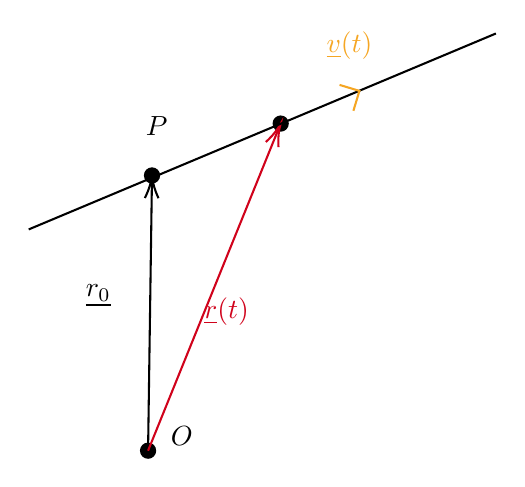
\begin{tikzpicture}[x=0.75pt,y=0.75pt,yscale=-1,xscale=1]
		%uncomment if require: \path (0,402); %set diagram left start at 0, and has height of 402

		%Straight Lines [id:da07486429812279405] 
		\draw    (203.5,258.3) -- (205.37,127.7) ;
		\draw [shift={(205.4,125.7)}, rotate = 90.82] [color={rgb, 255:red, 0; green, 0; blue, 0 }  ][line width=0.75]    (10.93,-3.29) .. controls (6.95,-1.4) and (3.31,-0.3) .. (0,0) .. controls (3.31,0.3) and (6.95,1.4) .. (10.93,3.29)   ;
		%Shape: Circle [id:dp6919219182514531] 
		\draw  [fill={rgb, 255:red, 0; green, 0; blue, 0 }  ,fill opacity=1 ] (202,125.7) .. controls (202,123.82) and (203.52,122.3) .. (205.4,122.3) .. controls (207.28,122.3) and (208.8,123.82) .. (208.8,125.7) .. controls (208.8,127.58) and (207.28,129.1) .. (205.4,129.1) .. controls (203.52,129.1) and (202,127.58) .. (202,125.7) -- cycle ;
		%Shape: Circle [id:dp2798104629473662] 
		\draw  [fill={rgb, 255:red, 0; green, 0; blue, 0 }  ,fill opacity=1 ] (200.1,258.3) .. controls (200.1,256.42) and (201.62,254.9) .. (203.5,254.9) .. controls (205.38,254.9) and (206.9,256.42) .. (206.9,258.3) .. controls (206.9,260.18) and (205.38,261.7) .. (203.5,261.7) .. controls (201.62,261.7) and (200.1,260.18) .. (200.1,258.3) -- cycle ;
		%Shape: Circle [id:dp4797202017377725] 
		\draw  [fill={rgb, 255:red, 0; green, 0; blue, 0 }  ,fill opacity=1 ] (264,100.7) .. controls (264,98.82) and (265.52,97.3) .. (267.4,97.3) .. controls (269.28,97.3) and (270.8,98.82) .. (270.8,100.7) .. controls (270.8,102.58) and (269.28,104.1) .. (267.4,104.1) .. controls (265.52,104.1) and (264,102.58) .. (264,100.7) -- cycle ;
		%Straight Lines [id:da797119100975235] 
		\draw [color={rgb, 255:red, 208; green, 2; blue, 27 }  ,draw opacity=1 ]   (203.5,258.3) -- (266.65,102.55) ;
		\draw [shift={(267.4,100.7)}, rotate = 112.07] [color={rgb, 255:red, 208; green, 2; blue, 27 }  ,draw opacity=1 ][line width=0.75]    (10.93,-3.29) .. controls (6.95,-1.4) and (3.31,-0.3) .. (0,0) .. controls (3.31,0.3) and (6.95,1.4) .. (10.93,3.29)   ;
		%Straight Lines [id:da8657231564938234] 
		\draw    (146,151.7) -- (371.1,57.3) ;
		%Shape: Right Angle [id:dp4402177451309871] 
		\draw  [color={rgb, 255:red, 245; green, 166; blue, 35 }  ,draw opacity=1 ] (295.76,82.07) -- (305.33,84.96) -- (302.44,94.53) ;

		% Text Node
		\draw (213,245) node [anchor=north west][inner sep=0.75pt]   [align=left] {$\displaystyle O$};
		% Text Node
		\draw (201,96) node [anchor=north west][inner sep=0.75pt]   [align=left] {$\displaystyle P$};
		% Text Node
		\draw (172,177) node [anchor=north west][inner sep=0.75pt]   [align=left] {$\displaystyle \underline{r_{0}}$};
		% Text Node
		\draw (229,183) node [anchor=north west][inner sep=0.75pt]  [color={rgb, 255:red, 208; green, 2; blue, 27 }  ,opacity=1 ] [align=left] {$\displaystyle \underline{r}( t)$};
		% Text Node
		\draw (288,55) node [anchor=north west][inner sep=0.75pt]  [color={rgb, 255:red, 245; green, 166; blue, 35 }  ,opacity=1 ] [align=left] {$\displaystyle \underline{v}( t)$};


	\end{tikzpicture}
\end{mycenter}

Using Vector equation of Lines (\ref{eq: vector-lines}), we get the following equation for $\underline{r}(t)$
$$\underline{r}(t) = \underline{r_{0}} + t\underline{v} \ \ \ \ \ \ \ \ \ \ \ \ \ \underline{v}, \underline{r_{0}}\ \ \ \text{are constants}$$
Then we can find the Velocity (\ref{eq: velocity-particle}) and Acceleration as (\ref{eq: acceleration-particle}) as
$$\begin{aligned}                          & \underline{v}(t) = \frac{d\underline{r}(t)}{dt} = \underline{\dot{r}}(t) = \underline{v}        \\ \\
                                         & \underline{a}(t) = \frac{d\underline{\dot{r}}(t)}{dt} = \ddot{\underline{r}(t)} = \underline{0}\end{aligned}$$

\subsubsection{Parabolic Trajectory}
\begin{definition}[Parabolic Trajectory]
	A parabolic trajectory is defined as
	\begin{equation}
		\label{eq: parabolic-trajectory}
		\underline{r} = \underline{r_{0}}+ \underline{v}_{0}t + \underline{a_{0}}\frac{1}{2}t^2
	\end{equation}
	where $\underline{v_0}$ and $\underline{r_0}$ are constants
\end{definition}
Acceleration (\ref{eq: acceleration-particle}) and Velocity (\ref{eq: velocity-particle}) are
\begin{itemize}
	\item $\displaystyle \underline{v}(t) = \frac{d\underline{r}(t)}{dt} = \underline{\dot{r}}(t) = \underline{v_{0}} + \underline{a_{0}}t$
	\item $\displaystyle \underline{a}(t) = \underline{\dot{v}}(t) = \frac{d}{dt}(\underline{v_{0}} + \underline{a_{0}}t) = \underline{a_0}$
\end{itemize}

{\bf Example of a Parabolic Trajectory:}
Consider the following equation:
$$\underline{r}(t) = (\underbrace{u_{0}\underline{i} + v_{0}\underline{k}}_{\underline{v_{0}}}) - \frac{1}{2}gt^{2}\underline{k}$$

\begin{mycenter}
	\tikzset{every picture/.style={line width=0.75pt}} %set default line width to 0.75pt        

	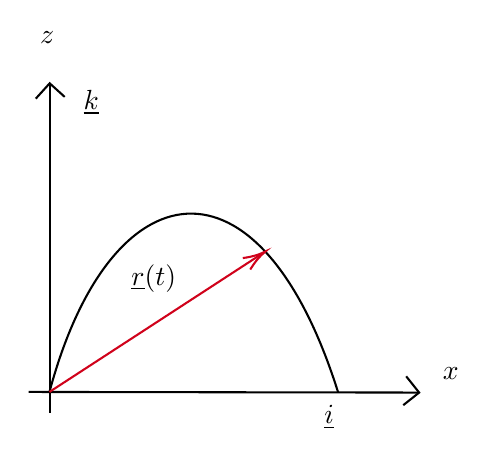
\begin{tikzpicture}[x=0.75pt,y=0.75pt,yscale=-1,xscale=1]
		%uncomment if require: \path (0,402); %set diagram left start at 0, and has height of 402

		%Straight Lines [id:da021686159454420983] 
		\draw    (150.1,91.3) -- (150.1,250.3) ;
		%Straight Lines [id:da9865222157984955] 
		\draw    (140,240) -- (328.1,240.3) ;
		%Shape: Right Angle [id:dp4412444494112757] 
		\draw   (143.39,98.71) -- (150.1,91.3) -- (157.33,97.84) ;
		%Shape: Right Angle [id:dp7802119319801154] 
		\draw   (321.88,232.47) -- (328.1,240.3) -- (320.46,246.37) ;
		%Curve Lines [id:da14645678527741524] 
		\draw    (150,240) .. controls (179.1,131.3) and (251.2,119.6) .. (289.1,240.3) ;
		%Straight Lines [id:da915058268090938] 
		\draw [color={rgb, 255:red, 208; green, 2; blue, 27 }  ,draw opacity=1 ]   (150,240) -- (252.42,173.39) ;
		\draw [shift={(254.1,172.3)}, rotate = 146.96] [color={rgb, 255:red, 208; green, 2; blue, 27 }  ,draw opacity=1 ][line width=0.75]    (10.93,-3.29) .. controls (6.95,-1.4) and (3.31,-0.3) .. (0,0) .. controls (3.31,0.3) and (6.95,1.4) .. (10.93,3.29)   ;

		% Text Node
		\draw (188,177) node [anchor=north west][inner sep=0.75pt]   [align=left] {$\displaystyle \underline{r}( t)$};
		% Text Node
		\draw (165,93) node [anchor=north west][inner sep=0.75pt]   [align=left] {$\displaystyle \underline{k}$};
		% Text Node
		\draw (144,65) node [anchor=north west][inner sep=0.75pt]   [align=left] {$\displaystyle z$};
		% Text Node
		\draw (281,245) node [anchor=north west][inner sep=0.75pt]   [align=left] {$\displaystyle \underline{i}$};
		% Text Node
		\draw (338,227) node [anchor=north west][inner sep=0.75pt]   [align=left] {$\displaystyle x$};


	\end{tikzpicture}
\end{mycenter}

Here, separating the {\bf components} if $\underline{i}$ and $\underline{k}$, we get the following ({\bf scalars}):
$$
	{x}(t) = u_{0}t \Rightarrow t = \frac{x(t)}{u_{0}}
$$
and substituting for in the value for $z(t)$ (component of $\underline{k}$),
$$\begin{aligned} z & = {v_{0}t} - \frac{1}{2}gt^{2 }                                           \\ \\
                  & = \frac{v_{0}\ x}{u_{0}} - \frac{1}{2}g\Big(\frac{x}{u_{0}}\Big)^{2 }     \\ \\
                  & = \frac{v_{0} \ x}{u_{0}}\Big(1 - \frac{1}{2}\frac{gx}{u_{0}\ v_{0}}\Big)\end{aligned}$$
And therefore as we can see, the equation for $z(t)$ is in the form of a {\bf parabola}.

\subsubsection{Circular Trajectory}
\begin{definition}[Circular Trajectory]
	Consider a particle {\bf trajectory} by the described by the following equations
	\begin{equation}
		\label{eq: circular-trajectory}
		\underline{r}(t) = a(\cos(\omega t)\underline{i} + \sin(\omega t)\underline{j})
	\end{equation}
\end{definition}

\begin{itemize}
	\item $x(t) = a\cos(\omega t)$ i.e. the $x$-component
	\item $y(t) = a\sin(\omega t)$ i.e. the $y$-component
\end{itemize}

\begin{note}
	$$x^{2}+ y^{2} = a^{2}\cos^{2}(\omega t) + a^{2}\cos^{2}(\omega t) \ \ \ \Rightarrow \ \ \  x^{2} + y^{2} = a^{2}$$
	which is the {\bf equation of a circle} of radius $a$.

\end{note}

{\bf Velocity in a circular trajectory}

First calculating the Velocity (\ref{eq: velocity-particle}),
$$\underline{\dot{r}}(t) = a(-\omega \sin(\omega t)\underline{i} + \omega\cos(\omega t)\underline{j})$$
where:
\begin{itemize}
	\item $\dot{x}(t) = -a\ \omega\sin(\omega t)$ i.e. the velocity in $x$-direction
	\item $\dot{y}(t) = a\ \omega\cos(\omega t)$ i.e. the velocity in $y$-direction
\end{itemize}
The {\bf magnitude} of velocity is:
$$\begin{aligned} \mid \underline{\dot{r}} \mid^{2} & = x^{2} + y^{2}                                                         \\ \\
                                                  & = a^{2}\omega^{2}\sin^{2}(\omega t) + a^{2}\omega^{2}\cos^{2}(\omega t) \\ \\
                                                  & = a^{2} \omega^{2}                                                      \\
                \Rightarrow\mid\underline{\dot{r}}\mid =  \mid\underline{v}\mid =a\omega\end{aligned}$$
We can see that velocity has a {\bf constant magnitude}, but is clearly {\bf changing in direction}.
The particle is moving in the {\bf anti-clockwise} direction. (This can be verified by \emph{checking any random point}).

	{\bf Acceleration in a circular trajectory}
Calculating the Acceleration (\ref{eq: acceleration-particle}),

$$\begin{aligned} \underline{\ddot{r}}(t) & = -a\omega^{2}(\cos(\omega t)\underline{i} + \sin(\omega t)\underline{j}) \\ \\
                                        & = -\omega^{2}\underline{r}\end{aligned}$$
So as we can see from the equation $\underline{\ddot{r}}(t) = -\omega^{2}\underline{r}$, we can see that the acceleration points downwards, i.e. opposite to the direction of $\underline{r}$ i.e. position vector.


\begin{figure}[H]
\centering
\tikzset{every picture/.style={line width=0.75pt}} %set default line width to 0.75pt        
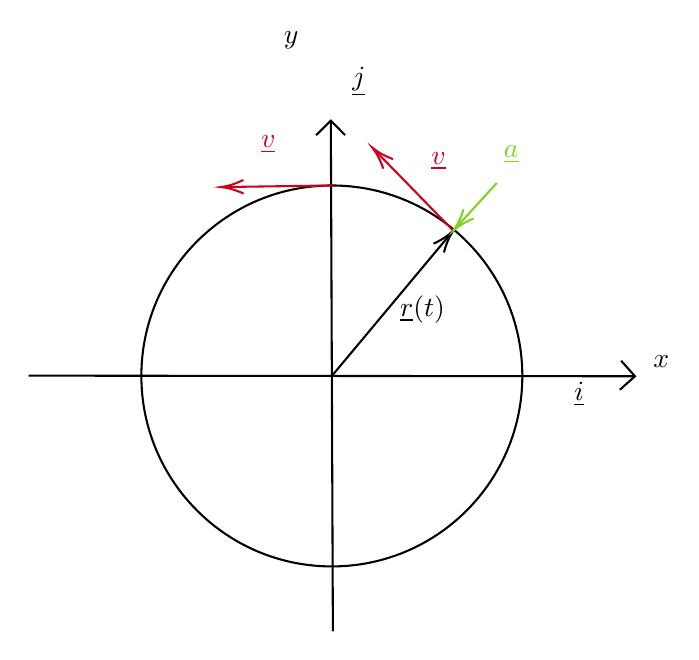
\begin{tikzpicture}[x=0.75pt,y=0.75pt,yscale=-1,xscale=1]
%uncomment if require: \path (0,402); %set diagram left start at 0, and has height of 402

%Straight Lines [id:da021686159454420983] 
\draw    (230.1,98.3) -- (231.1,344.3) ;
%Straight Lines [id:da9865222157984955] 
\draw    (84.55,221.15) -- (376.65,221.45) ;
%Shape: Right Angle [id:dp4412444494112757] 
\draw   (222.98,105.32) -- (230.1,98.3) -- (236.95,105.24) ;
%Shape: Right Angle [id:dp7802119319801154] 
\draw   (369.99,213.99) -- (376.65,221.45) -- (369.37,227.94) ;
%Shape: Circle [id:dp5189182370807889] 
\draw   (138.82,221.3) .. controls (138.82,170.61) and (179.91,129.53) .. (230.6,129.53) .. controls (281.29,129.53) and (322.37,170.61) .. (322.37,221.3) .. controls (322.37,271.99) and (281.29,313.07) .. (230.6,313.07) .. controls (179.91,313.07) and (138.82,271.99) .. (138.82,221.3) -- cycle ;
%Straight Lines [id:da030770231855278496] 
\draw [color={rgb, 255:red, 208; green, 2; blue, 27 }  ,draw opacity=1 ]   (230.6,129.53) -- (179.1,130.27) ;
\draw [shift={(177.1,130.3)}, rotate = 359.17] [color={rgb, 255:red, 208; green, 2; blue, 27 }  ,draw opacity=1 ][line width=0.75]    (10.93,-3.29) .. controls (6.95,-1.4) and (3.31,-0.3) .. (0,0) .. controls (3.31,0.3) and (6.95,1.4) .. (10.93,3.29)   ;
%Straight Lines [id:da00482572515300661] 
\draw [color={rgb, 255:red, 208; green, 2; blue, 27 }  ,draw opacity=1 ]   (289.1,151.3) -- (251.5,112.73) ;
\draw [shift={(250.1,111.3)}, rotate = 45.73] [color={rgb, 255:red, 208; green, 2; blue, 27 }  ,draw opacity=1 ][line width=0.75]    (10.93,-3.29) .. controls (6.95,-1.4) and (3.31,-0.3) .. (0,0) .. controls (3.31,0.3) and (6.95,1.4) .. (10.93,3.29)   ;
%Straight Lines [id:da678334264237589] 
\draw    (230.6,221.3) -- (287.82,152.83) ;
\draw [shift={(289.1,151.3)}, rotate = 129.89] [color={rgb, 255:red, 0; green, 0; blue, 0 }  ][line width=0.75]    (10.93,-3.29) .. controls (6.95,-1.4) and (3.31,-0.3) .. (0,0) .. controls (3.31,0.3) and (6.95,1.4) .. (10.93,3.29)   ;
%Straight Lines [id:da503332446941831] 
\draw [color={rgb, 255:red, 126; green, 211; blue, 33 }  ,draw opacity=1 ]   (310.1,128.3) -- (290.45,149.82) ;
\draw [shift={(289.1,151.3)}, rotate = 312.4] [color={rgb, 255:red, 126; green, 211; blue, 33 }  ,draw opacity=1 ][line width=0.75]    (10.93,-3.29) .. controls (6.95,-1.4) and (3.31,-0.3) .. (0,0) .. controls (3.31,0.3) and (6.95,1.4) .. (10.93,3.29)   ;

% Text Node
\draw (262,181) node [anchor=north west][inner sep=0.75pt]   [align=left] {$\displaystyle \underline{r}( t)$};
% Text Node
\draw (239,71) node [anchor=north west][inner sep=0.75pt]   [align=left] {$\displaystyle \underline{j}$};
% Text Node
\draw (206,54) node [anchor=north west][inner sep=0.75pt]   [align=left] {$\displaystyle y$};
% Text Node
\draw (346,223) node [anchor=north west][inner sep=0.75pt]   [align=left] {$\displaystyle \underline{i}$};
% Text Node
\draw (384,210) node [anchor=north west][inner sep=0.75pt]   [align=left] {$\displaystyle x$};
% Text Node
\draw (195,104) node [anchor=north west][inner sep=0.75pt]  [color={rgb, 255:red, 208; green, 2; blue, 27 }  ,opacity=1 ] [align=left] {$\displaystyle \underline{v}$};
% Text Node
\draw (277,112) node [anchor=north west][inner sep=0.75pt]  [color={rgb, 255:red, 208; green, 2; blue, 27 }  ,opacity=1 ] [align=left] {$\displaystyle \underline{v}$};
% Text Node
\draw (312,109) node [anchor=north west][inner sep=0.75pt]  [color={rgb, 255:red, 126; green, 211; blue, 33 }  ,opacity=1 ] [align=left] {$\displaystyle \underline{a}$};


\end{tikzpicture}
\caption{Circular Trajectory} \label{fig: circular-trajectory-diagram}
\end{figure}

\clearpage
